\documentclass[a4paper]{article}
\usepackage[warn]{mathtext}
\usepackage[utf8]{inputenc}
\usepackage[T2A]{fontenc}
\usepackage[english,russian]{babel}
\usepackage{indentfirst}
\usepackage{misccorr}
\usepackage{subcaption}
\captionsetup{compatibility=false}
\usepackage{geometry}
\geometry{verbose,a4paper,tmargin=2cm,bmargin=2cm,lmargin=1.5cm,rmargin=1.5cm}
\usepackage{graphicx}
\usepackage{wrapfig}
\usepackage{amsmath}
\usepackage{fancyhdr}
\usepackage{floatflt}
\usepackage{float}
\usepackage{amssymb}
\usepackage{color}
\usepackage{lscape}
\usepackage{hvfloat}
\usepackage{amsfonts}
\usepackage{euscript}
\usepackage{newunicodechar}
\usepackage{booktabs}
\usepackage{epigraph}
\usepackage{csquotes} 
\usepackage{hyperref}

\hypersetup{
    colorlinks=true,      
    urlcolor=blue,
    linkcolor= blue
}

\begin{document}
\newcommand{\apple}{\char"F8FF}



% \begin{titlepage}
%     \vspace*{4cm}
% 	\centering
%     {\scshape\LARGE Московский физико-технический институт\par}
% 	\vspace{1cm}
% 	{\scshape\Large Дипломная работа\par}
% 	\vspace{1cm}
%     {\huge\bfseries Реализация взаимодействия мобильных агентов в mesh-сети,  обладающей  локальными свойствами. \par}
% 	\vspace{2cm}
% 	\vfill
% \begin{flushright}
% 	{\large Выполнила студентка Б01-907}\par
% 	\vspace{0.3cm}
% 	{\LARGE Юлия Прохорова}
% \end{flushright}
	
% 	\vfill
% Долгопрудный, 2023
% % Bottom of the page
% \end{titlepage}

\pagestyle{fancy} 
\fancyhead[L]{Дипломная работа}
\fancyhead[R]{Юлия Прохорова, Б01-907}
\fancyhead[C]{}
\fancyfoot[C]{ \noindent\rule{\textwidth}{0.4pt} \thepage }

\tableofcontents

\newpage

\epigraph{Mesh: пространство или промежуток между нитями сети.}{Новый английский словарь (М.: Oxford Press, 1932)}

\section{Введение и постановка задачи}
Введем понятие \textbf{сети} как набора объектов (вершин), связанных между собой. Иллюстрацию данного определения можно увидеть на на рис.\ref{p1}. Существуют различные виды сетей: общественные сети, информационные, биологические и т.д. \par
Также сети различают по их \textbf{топологиям} - путям передачи данных в сети (?вообще есть физическая и логическая топология - мы рассматриваем именно логическую?):

\begin{figure}[H]
	\begin{center}
	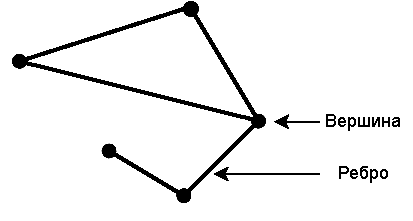
\includegraphics[width=0.4\linewidth]{net.pdf}
	\caption{Пример сети.} 
    \label{p1}
    \end {center}
\end{figure}

\begin{itemize}
    \item Ячеистая (mesh) - каждое устройство подключается к другому устройству через определенный канал;
    \item Топология шины - к кабелю, который выступает в качестве общей разделяемой среды передачи данных, подключены все устройства;
    \item Кольцевая топология - каждое устройство соединяется ровно с двумя соседними, а вместе они образуют кольцо;
    \item Топология звезды - все устройства подключаются к одному сетевому устройству;
    \item Гибридная топология - комбинация различных топологий;
\end{itemize}
В данной работе будут рассматриваться только mesh-сети.
\subsection{Mesh-сети}
Как отображено на pис.\ref{p2}, в mesh-сети все устройства связаны друг с другом через определенный канал.
Mesh-сети бывают: 
\begin{itemize}
    \item Полносвязными (full-mesh);
    \item Неполносвязными (partial-mesh).
\end{itemize}

\begin{figure}[H]
    \text{a)}
	\begin{minipage}[h]{0.45\linewidth}
	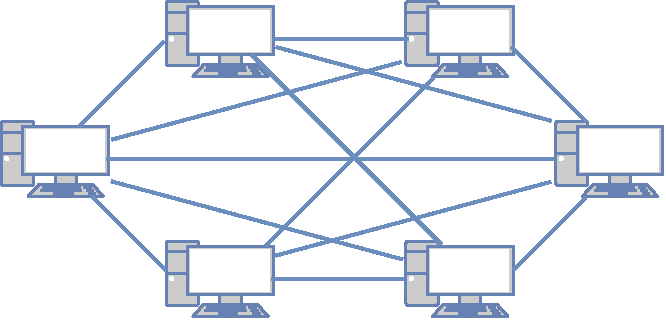
\includegraphics[width=1\linewidth]{full.pdf}
	\end{minipage}
	\hfill 
    \text{b)}
	\begin{minipage}[h]{0.43\linewidth}
	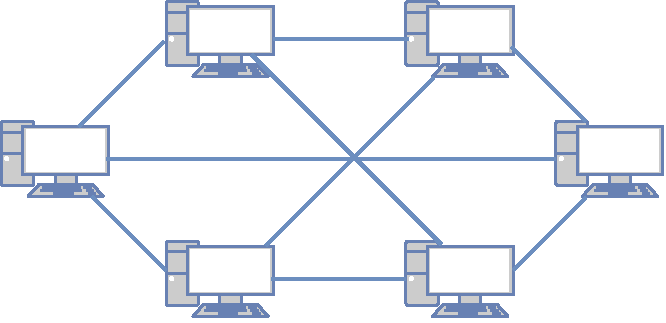
\includegraphics[width=1\linewidth]{partial.pdf}
	\end{minipage}
    \caption{\\a) \;Full-mesh сеть. b)\; Partial-mesh сеть.}
    \label{p2}
\end{figure}

\textbf{Полноcвязная топология} \par

В данной топологии все узлы в сети связаны друг с другом. Если в сети имеется $N$ узлов, каждый узел будет иметь $N-1$ соединений.
 Полносвязная сеть обеспечивает превосходную степень избыточности, но поскольку ее реализация будет дороже, чем у неполносвязной, ее обычно резервируют для сетевых магистралей.
 
\textbf{Неполносвязная топология}

В частично связанной сети не обязательно все узлы связаны друг с другомы. Она более практична по сравнению с full-mesh. 
Периферийные сети подключаются с использованием неполносвязной сети и подключаются к полноячеистой магистральной сети.

Топология Mesh основана на децентрализованной схеме организации сети, в отличие от типовых сетей, которые создаются по централизованному принципу.
 Точки доступа, работающие в Mesh-сетях, не только предоставляют услуги абонентского доступа, но и выполняют функции маршрутизаторов/ретрансляторов для других точек доступа той же сети. 

Mesh-сети строятся как совокупность кластеров - зон. Территория, которая покрыта сетями, разделяется на кластерные зоны, число которых теоретически не ограничено. 
Особенностью такой сети является использование специальных протоколов, позволяющих каждой точке доступа создавать таблицы абонентов сети с контролем состояния транспортного канала и поддержкой динамической маршрутизации трафика по оптимальному маршруту между соседними узлами. 
При отказе какого-либо из них происходит автоматическое перенаправление трафика по другому маршруту, что гарантирует не просто доставку трафика адресату, а доставку за минимальное время.

Процедура расширения сети в пределах кластера ограничивается установкой новых точек доступа, интеграция которых в существующую сеть происходит автоматически.

\subsection{Безопасность Mesh-сетей}

Вопросы безопасности Mesh  являются весьма актуальными, особенно для систем городского масштаба, которые объединяют муниципальные, абонентские и корпоративные сети. 
Безопасность сетей обеспечивается в рамках спецификаций стандарта 802.11. Стандарт IEEE 802.11i предусматривает использование в продуктах Wi-Fi таких средств, как поддержка алгоритмов шифрования трафика: TKIP, WRAP и CCMP.
 Этих алгоритмов достаточно для защиты на уровне абонентского трафика, но на уровне корпоративного пользователя используются дополнительные механизмы, включающие более совершенные способы аутентификации при подключении к сети: более крипто-стойкие методы шифрования, динамическую замену ключей шифрования, использование персональных межсетевых экранов, мониторинг защищенности беспроводной сети, технологию виртуальных частных сетей VPN и т.д.
\\

 Основываясь на статье \href{https://www.geeksforgeeks.org/advantage-and-disadvantage-of-mesh-topology/}{Преимущества и недостатки ячеистой топологии} можно сделать следующие выводы:
 \subsection[]{Преимущества ячеистой топологии}

\begin{itemize}
    \item В случае сбоя одного устройства - сеть продолжит функционировать в том же режиме.
    \item Просто локализовать неисправность.
    \item Передача данных более стабильна, так как сбои не выводит всю систему из строя - передача данных реализуется другим путем.
    \item Проблем с трафиком нет, так как для каждого компьютера есть выделенная двухточечная связь.
    \item Эта топология обеспечивает несколько путей для достижения нужного узла и соответственно хорошую устойчивость.
    \item Добавление новых устройств не нарушает передачу данных.
\end{itemize}

\subsection[]{Недостатки ячеистой топологии}
\begin{itemize}
    \item Реализация такой сети дороже по сравнению с иными сетевыми топологиями, т.е. звездой, шиной, двухточечной топологией.
    \item Требуемая мощность оборудования должна быть выше, так как узлы остаются активными все время и распределяют нагрузку между собой.
    \item Некоторые устройства будут избыточными в схеме передачи данных.
\end{itemize}

\section{Сети малого мира}
В статье "Mean-field solution of the small-world network model" M. E. J. Newman, C. Moore, and D. J. Watts сети малого мира описываюся по аналогии с сетью друзей. 
В сети друзей присутствует “кластеризация”, означающая, что двое ваших друзей с гораздо большей вероятностью также будут друзьями друг друга, чем два человека, выбранных случайным образом из популяции. 
Во-вторых, такая сеть демонстрирует “эффект маленького мира”, а именно, что любые два человека могут установить контакт, пройдя лишь короткую цепочку промежуточных знакомств. 
Американский психолог Милграм провел интересное исследование, котором определил количество знакомств, необходимое для установления связи между данными людьми. Поскольку Милграм жил в Бостоне, он выбран далекий от Бостона город - Небраска, 
и случайно выбранным людям были розданы конверты, которые нужно было передать в Бостон. Конверты можно было передавать только через своих знакомых и родственников. Милграм получил весьма неожиданный результат: 
в среднем каждый конверт прошел через шесть человек. Так и родилась теория "шести рукопожатий". Т.е. каждый человек связан с любым другим цепью не больше шести личных знакомств. В этом смысле о нашем мире говорят как о малом мире - "small world".

Модель перехода от большого мира к малому предложили Ваттс и Строгац. Эта модель представляет собой одномерную регулярную решетку, состоящую из $N$ узлов,
 где каждый узел соединен только со своими k ближайшими соседями и наложены периодические граничные условия, т.е. решетку свернули в кольцо. После чего каждую связь с вероятностью $\phi << C_1$ перебрасывали на другой случайно выбранный узел.
 Правда при такой процедуре есть вероятность появления изолированных узлов.

 \begin{figure}[H]
    \begin{center}
    \text{a)}
	\begin{minipage}[h]{0.4\linewidth}
	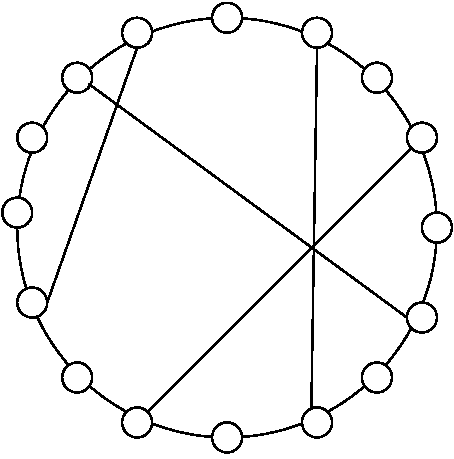
\includegraphics[width=1\linewidth]{2соседа.pdf}
	\end{minipage}
	\hfill 
    \text{b)}
	\begin{minipage}[h]{0.4\linewidth}
	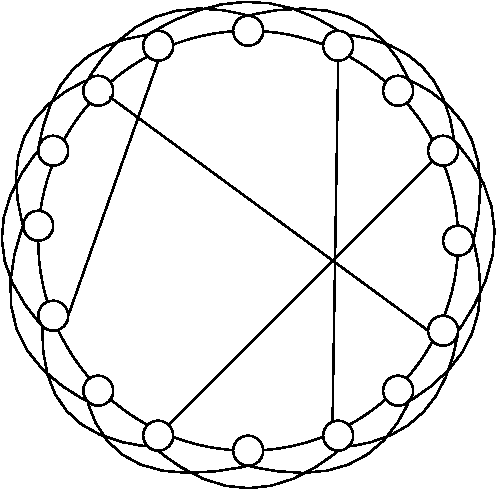
\includegraphics[width=1\linewidth]{3neighbours.pdf}
	\end{minipage}
        \caption{Пример малого мира с четырьмя перебросами ( $L = 16$) a) - каждый узел соединен со своими ближайшими соседями (к = 2), b) - каждый узел соединен с четырьмя соседями (к = 4)}
    \end{center}
    \label{p2}
\end{figure}

% Пусть $m (r)$ — количество узлов на графике, которые не являются соседними, усредненное по многим реализациям, а $n (r)$ - среднее число “кластеров” вокруг решетки, между которыми разделены эти узлы.
%  В модели континуума и m, и n являются действительными числами. Нам также будет удобно использовать масштабированные переменные: $\mu (r) = \frac{m(r)}{L}$, $\nu (r) = \frac{n(r)}{L}$.

%  В пределе континуума величины $m(r)$ и $n (r)$ удовлетворяют дифференциальным уравнениям следующим образом. Скорость, с которой количество пустых участков на решетке уменьшается с увеличением $r$, равна числу $2n$ растущих ребер кластеров на решетке, умноженному на диапазон $k$ соединений на решетке.
%   Таким образом, $\frac{dm}{dr}=-2kn$ или $\frac{d\mu}{dr} = -2k\nu$.

Формально расстояние до них от любого узла будет бесконечным. Во избежание этого, Ньюман (Newman) и Ваттс предложили связи не перебрасывать, а просто добавлять. Остановимся на этом варианте модели подробнее Среднее расстояние между концами добавленных
связей есть: $\xi = \frac{N}{k\phi N} = \frac{1}{k\phi}$.

Так как существует только один характерный размер системы $X$, то и безразмерное отношение среднего расстояния между узлами графа к числу всех узлов графа $N$ может зависеть только от безразмерной величины: $l = N f( \frac{N}{\xi})$, где $f(x)$ - скейлинговая функция. 
\begin{equation*}
    f(x) = 
    \begin{cases}
       cons, x \ll 1 \\
        \frac{\log(x)}{x}, x \gg 1
    \end{cases}
\end{equation*}

Как уже упоминалось выше, существует много способов определения корреляционного радиуса. Предположим, что $\xi \sim \phi^\tau$.
Покажем с помощью ренорм-группового преобразования (для к = 2), что Т = 1. Итак пусть имеем: $l = Nf(Nf^\tau)$.
\subsection{Примеры сетей малого мира}
Свойства маленького мира обнаруживаются во многих явлениях реального мира, включая веб-сайты с меню навигации, пищевые сети, электросети, сети обработки метаболитов, сети нейронов мозга , сети избирателей, телефонный звонок графики, сети аэропортов и социальные сети влияния. Культурные сети, семантические сети и словесные сети совместной встречаемости также оказались сетями небольшого мира.

Сети из связанных белков обладают свойствами небольшого мира, такими как степенное распределение, подчиняющееся распределению степеней. Точно так же транскрипционные сети , в которых узлами являются гены , и они связаны, если один ген оказывает повышающее или понижающее генетическое влияние на другой, обладают свойствами малых мировых сетей.

 \section{Обзор существующих моделей}
\section{Теоретическая часть работы}

\section[]{Реализация}
Даная исследователься работы нацелна создание макета обмена данных в группе мобильных агентов, взаимодействующих в mesh-сети обладающей свойствами “малого мира”.
Возможные технологии для реализации модели:
\begin{itemize}
    \item GNS3
    \item Docker
\end{itemize}
\section{Заключение}
\section{Литература}

\begin{thebibliography}{}
    \bibitem{litlink1}  M. E. J. Newman -  \href{https://github.com/julproh/Thesis}{The Structure and Function of Complex Networks}
    \bibitem{litlink2}  Geeks For Geeks -  \href{https://www.geeksforgeeks.org/advantage-and-disadvantage-of-mesh-topology/}{Advantage and Disadvantage of Mesh Topology}
    \bibitem{litlink2}  Осипов И.Е. -  \href{http://lib.tssonline.ru/articles2/fix-op/mesh_seti_techn_prilozh_oborud}{Технологии и средства связи \#4, 2006}
\end{thebibliography}
\end{document}

